\documentclass{beamer}
\PassOptionsToClass{handout}{beamer}


\usetheme{Madrid}

\usepackage{graphicx}
\usepackage{hyperref}
\usepackage{subcaption}
\usepackage{float}
\usepackage{csquotes}
\usepackage{pifont}
\setbeamertemplate{navigation symbols}{}
\usepackage[ngerman]{babel}
\usepackage[backend=bibtex]{biblatex}
\usepackage{algorithm}
\usepackage{algpseudocode}
\usepackage{tikz}
\usetikzlibrary{positioning}
\usepackage[absolute,overlay]{textpos}
\setbeamertemplate{footline}
{
  \leavevmode%
  \hbox{%
  \begin{beamercolorbox}[wd=.333333\paperwidth,ht=2.25ex,dp=1ex,center]{author in head/foot}%
    \usebeamerfont{author in head/foot}Ian Schmetkamp%\insertshortauthor
  \end{beamercolorbox}%
  \begin{beamercolorbox}[wd=.333333\paperwidth,ht=2.25ex,dp=1ex,center]{title in head/foot}%
    \usebeamerfont{title in head/foot}Autonomous Object Inspection
  \end{beamercolorbox}%
  \begin{beamercolorbox}[wd=.333333\paperwidth,ht=2.25ex,dp=1ex,right]{date in head/foot}%
    \usebeamerfont{date in head/foot}\insertshortdate{}\hspace*{2em}
    \insertframenumber{} / \inserttotalframenumber\hspace*{2ex}
  \end{beamercolorbox}}%
  \vskip0pt%
}
\date{}
\title{Autonomous Object Inspection with Mobile Robots for 3D Reconstruction and Image Data Acquisition}
%\author{Ian Schmetkamp \inst{1} \\ \textbf{Advisor:} Philip Keller \inst{2} \\ \textbf{Supervisor:} Prof. Dr.-Ing. Rüdiger Dillmann \inst{2}}
%\institute{\inst{1} Karlsruhe Institute of Technology \and \inst{2} FZI Research Center for Information Technology}

\bibliography{references.bib}
\begin{document}
\begin{frame}
	\centering
	\maketitle
	\vspace{-2cm}
	Ian Schmetkamp\footnotemark[1] \\ \textbf{Betreuende Personen:} Philip Keller\footnotemark[2] \\ Prof. Dr.-Ing. Dillmann\footnotemark[2] \\ Prof. Dr. Beckert\footnotemark[1]
	\vfill
	\footnotesize{ \footnotemark[1]Karlsruher Institute für Technologie \\  \footnotemark[2]Forschungszentrum Informatik}
	\vfill
	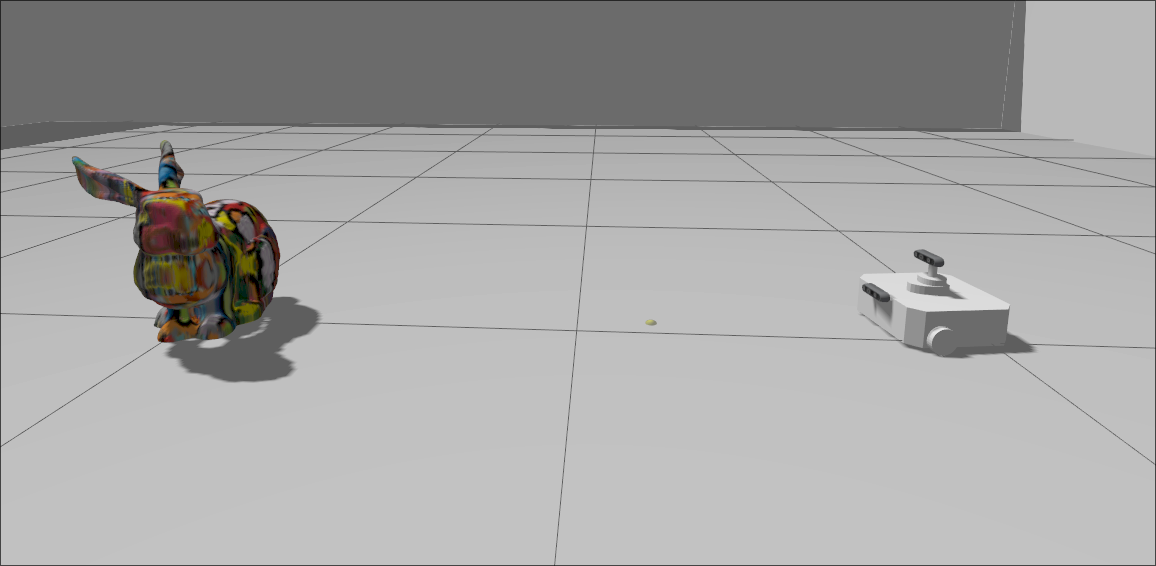
\includegraphics[width=0.5\textwidth]{Graphics/tbandbunny.png}

	\today
\end{frame}

\section{Allgemeines}
\begin{frame}{Motivation}
	\begin{minipage}{0.55 \textwidth}
		\begin{block}{Ziel}
			\begin{itemize}
				\item autonom Bilder von Objekt aufnehmen
				\item Bilder aus verschiedenen Perspektiven
				\item Bilder als Training für Perzeptionsmodellen
				\item Soll auf verschiedenen Robotern laufen (Spot, Turtlebot, etc.)
			\end{itemize}
		\end{block}
	\end{minipage}
	\hfill
	\begin{minipage}{0.4 \textwidth}
		\centering
		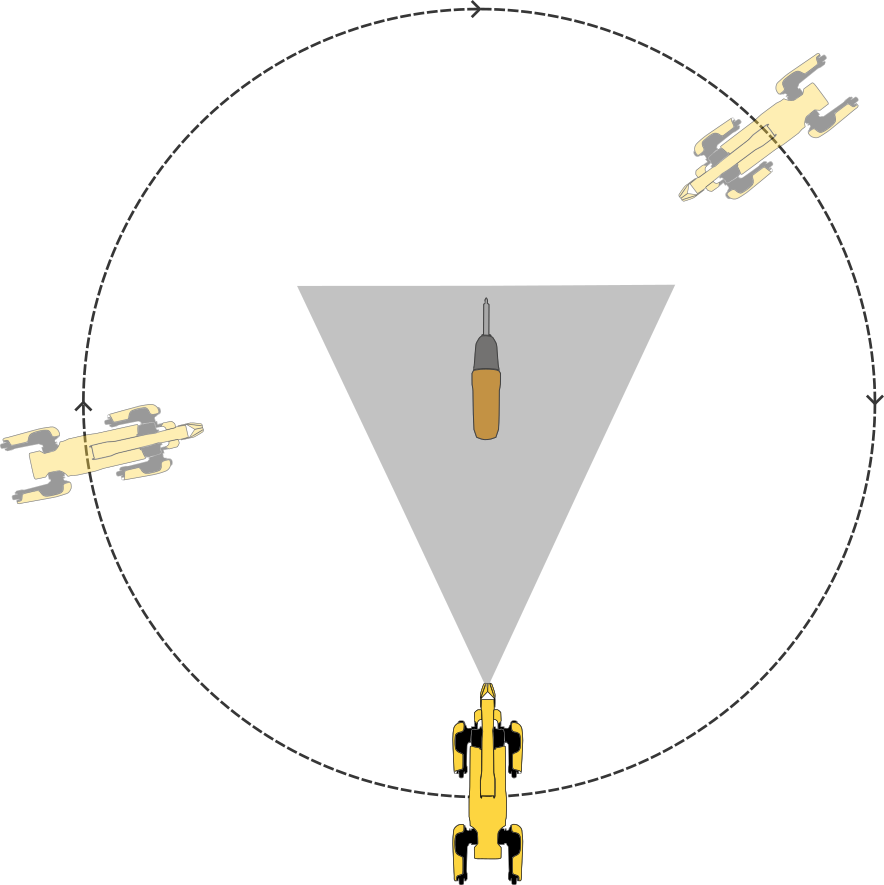
\includegraphics[width=1\textwidth]{Graphics/graphic_top_down.png}
	\end{minipage}
\end{frame}

\begin{frame}{State-of-the-Art}
	\begin{center}
		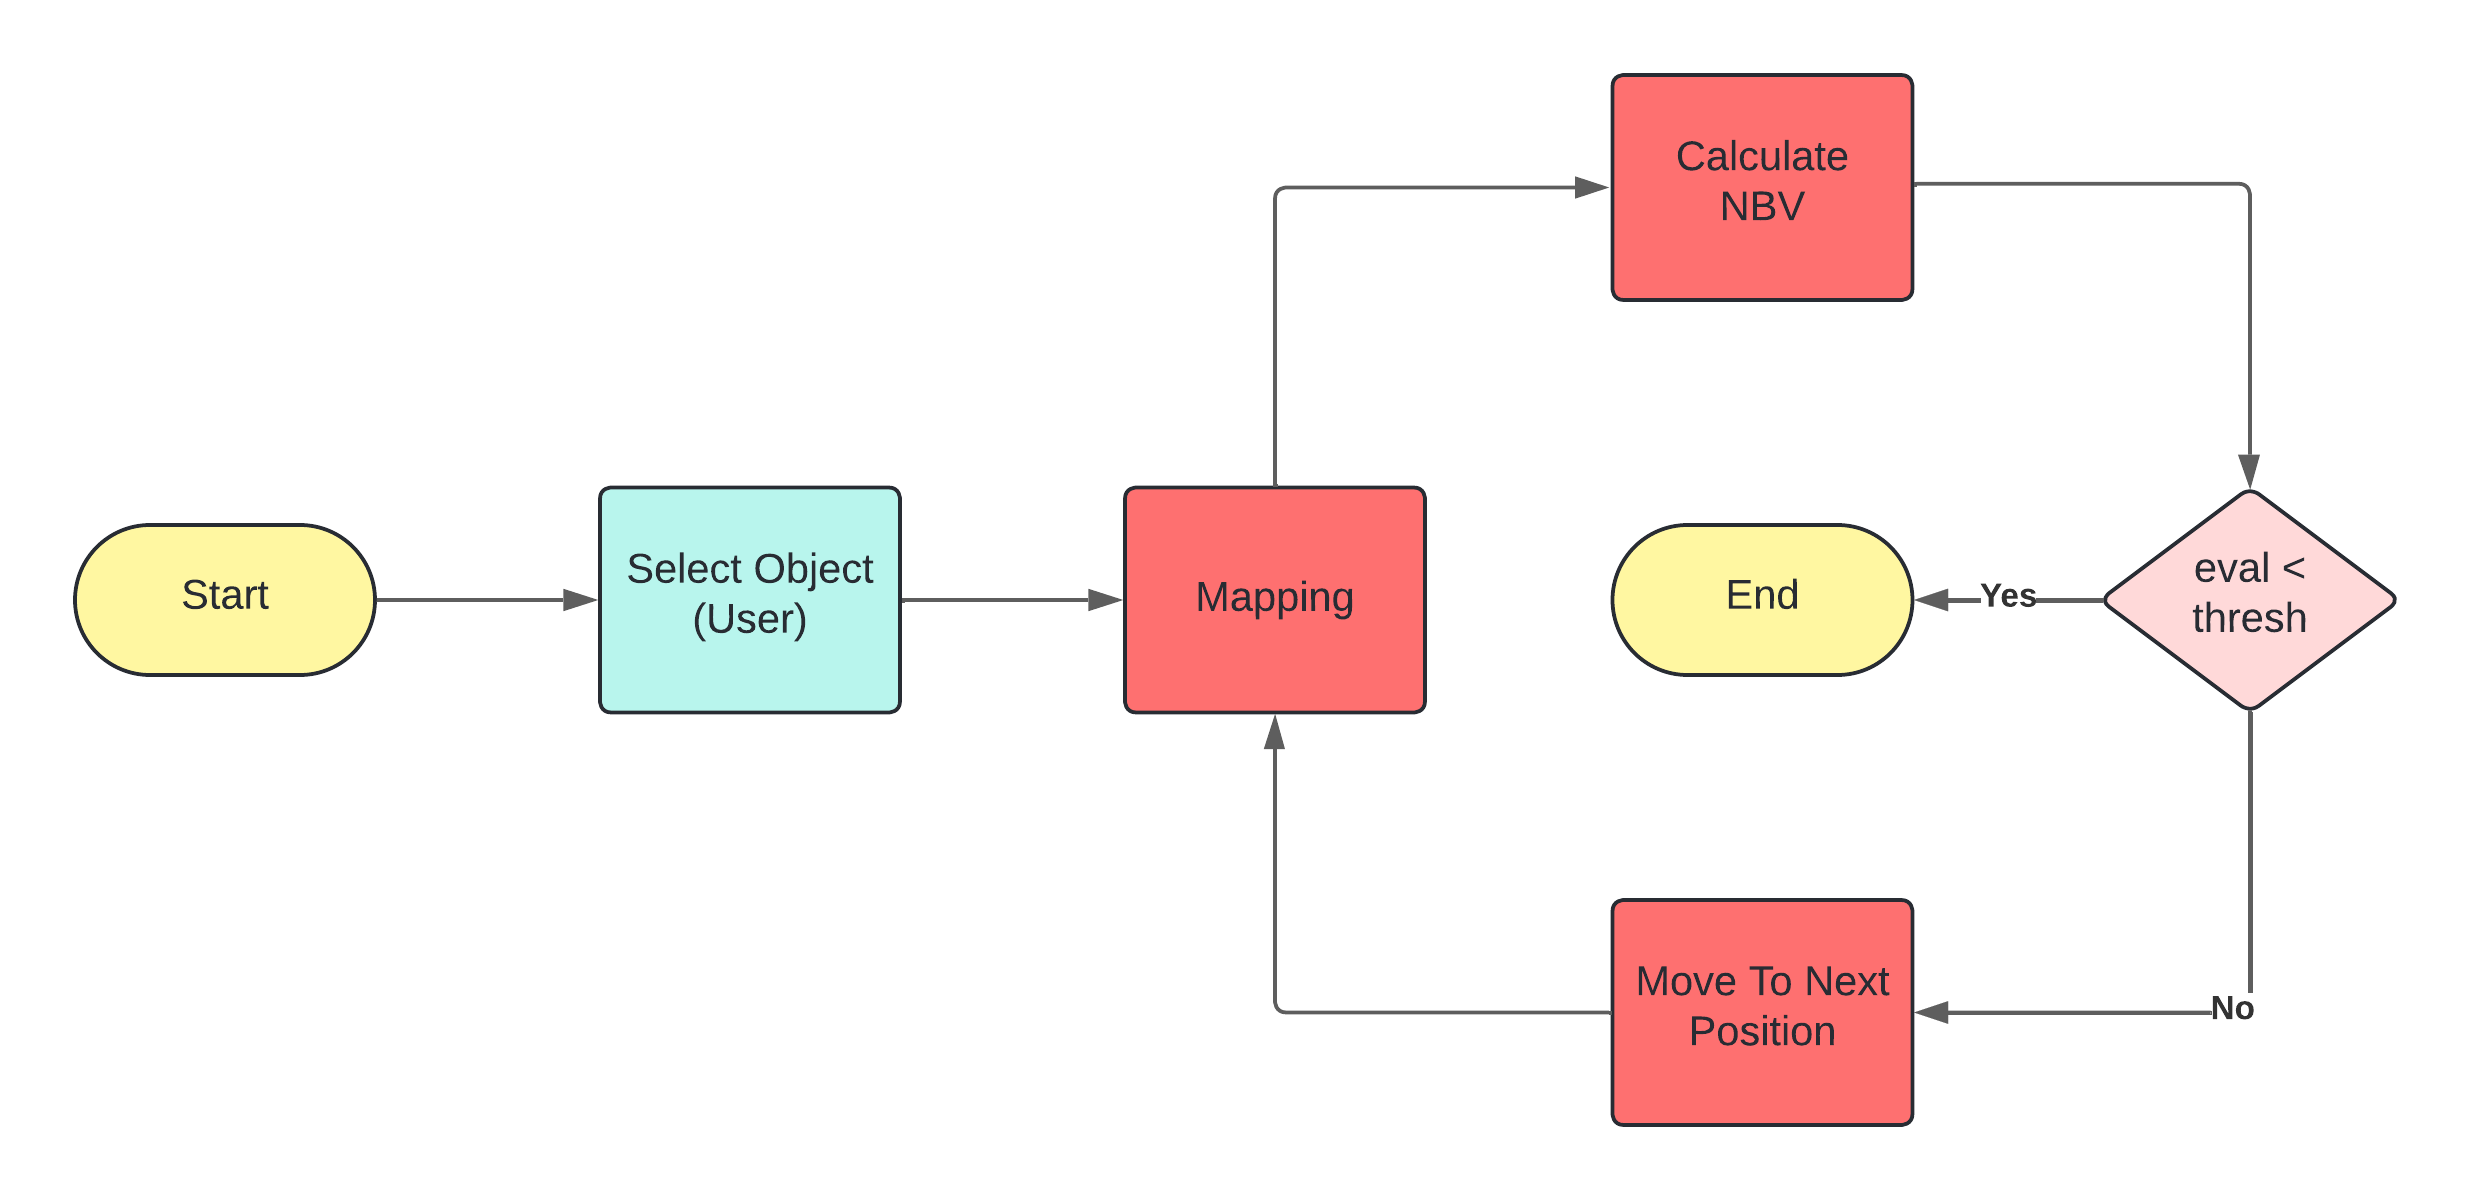
\includegraphics[width=0.65\textwidth]{Graphics/flow_chart.png}
	\end{center}

	\begin{block}{}
		\begin{itemize}
			\item Mögliche Positionen evaluieren
			\item Abschätzen wie viel Informationen in möglicher Position gesehen wird (Stichwort: Next-Best-View)
			\item Andere Faktoren für Positionen evaluieren (Distanz, Überlappung, Sichtbarkeit des Bekannten etc.)
			\item Zur besten Position gehen
		\end{itemize}
	\end{block}
\end{frame}

\section{State of the Art}
\begin{frame}{State-of-the-Art: NBV}
	\vspace{-1cm}
	\hfill
	\begin{minipage}{0.2\textwidth}
		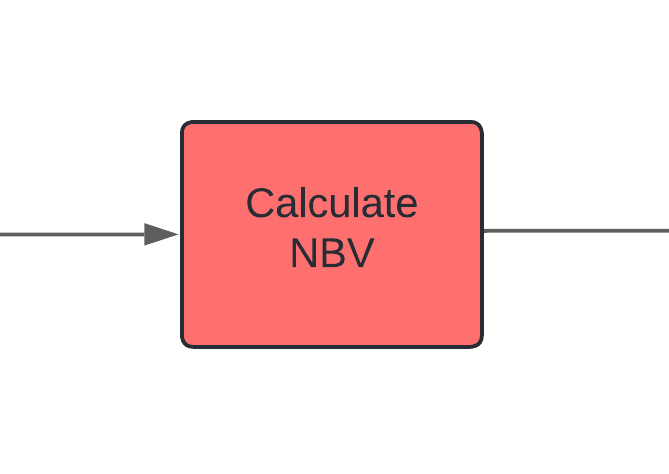
\includegraphics[width=\textwidth]{Graphics/nbv_flow.png}
	\end{minipage}
	\vspace{-0.5cm}
	\begin{block}{Klassische Ansätze}
		\begin{itemize}
			\item \textbf{Annahme:} Tiefensensor, Größe des Objekts bekannt (Bounding Box)
			\item Generierung von Kandidaten Sensorpose, meist auf Kugel um Objektzentrum
			\item Testen der Kandidaten auf \textbf{utility function}
			\item Zur besten Kandidaten Sensorpose bewegen
			\item \textbf{Repräsentation der Umgebung:} Octomap, ähnliche Voxelkarten
		\end{itemize}
		\cite{zeng_view_2020}
	\end{block}
	\begin{textblock*}{0.2\textwidth}(10cm, 6.5cm)
		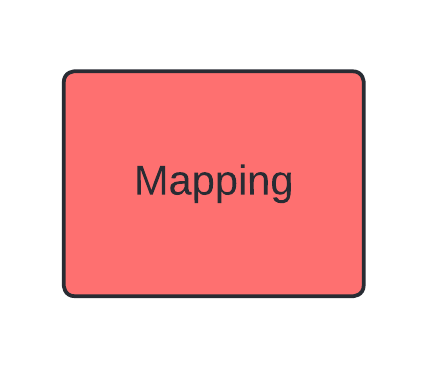
\includegraphics[width=\textwidth]{Graphics/mapping_flow.png}
	\end{textblock*}
\end{frame}

\begin{frame}{State-of-the-Art: NBV}
	\vspace{-1cm}
	\hfill
	\begin{minipage}{0.2\textwidth}
		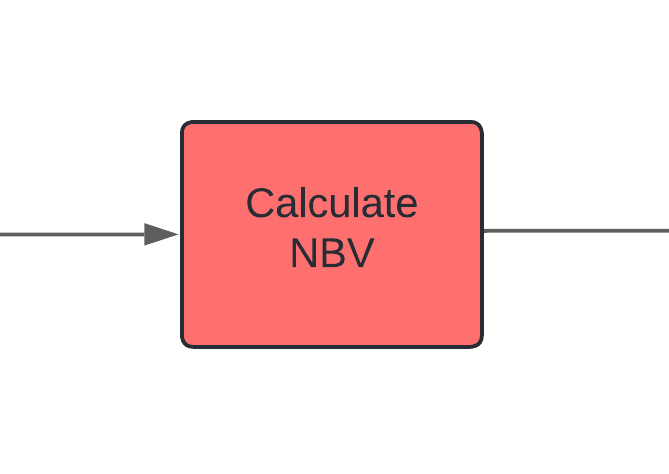
\includegraphics[width=\textwidth]{Graphics/nbv_flow.png}
	\end{minipage}
	\vspace{-0.5cm}
	\begin{block}{Machine-Learning Ansätze}
		\begin{itemize}
			\item \textbf{Annahme:} Trainingsdaten auf Basis von Punktwolke oder Voxelkarte
			\item Trainingsdaten enthalten nächst-beste Sensorpose für aktuelle Sensorpose
			\item Größe der Objekte meist fix
			\item Nächste Sensorpose vorhersagen
			\item PC-NBV \cite{zeng_pc-nbv_2020}, NBV-Net \cite{mendoza_supervised_2020}

		\end{itemize}
	\end{block}
\end{frame}

\begin{frame}{State-of-the-Art: Definitionen}
	\begin{exampleblock}{Visible unknown Voxel}
		\begin{itemize}
			\item unbekannte Voxel, die von einem anderen Punkt als erste gesehen werden
			\item unbekannte Voxel benachbart zu einem freien Voxel
		\end{itemize}
		\cite{vasquez-gomez_vpl_2020}
	\end{exampleblock}
	\begin{exampleblock}{Frontier Voxel}
		\begin{itemize}
			\item visible unknown Voxel, die benachbart zu besetzen Voxel sind
			\item benachbarte Frontier Voxel bilden eine Frontier

		\end{itemize}
		\cite{vasquez-gomez_vpl_2020}
	\end{exampleblock}
\end{frame}

\begin{frame}{}
	\begin{figure}
		\hspace{2.2cm}
		\begin{tikzpicture}
			% Centered image
			\node (main-image) at (current page.center) {
				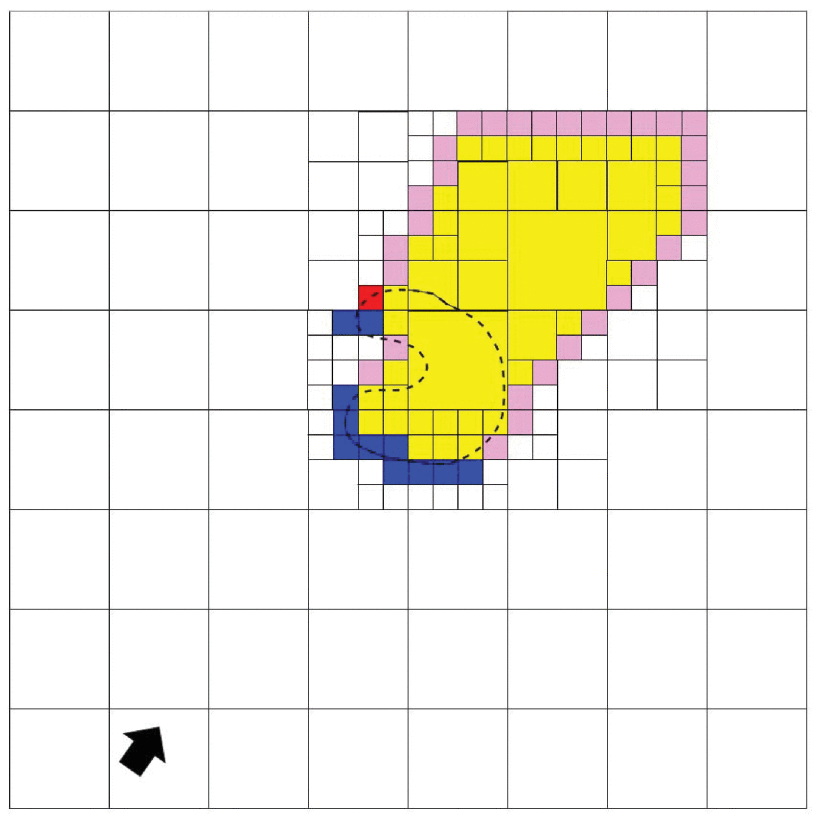
\includegraphics[width=6cm]{Graphics/vasquez.png} % Adjust width
			};
			% Secondary image at the top right of the centered image
			\node[xshift=1.5cm, yshift=-0.9cm]
			(secondary-image) at (main-image.north east){
				
\includegraphics[width=3cm]{Graphics/legend.png} % Smaller image
			};
		\end{tikzpicture}
		\caption{\cite{vasquez-gomez_vpl_2020}}
	\end{figure}
\end{frame}


\begin{frame}{Ansatz}
	\begin{block}{Besonderheiten}
		\begin{itemize}
			\item keine Information über Größe des Objekts
			\item VDB-Mapping statt OctoMap
		\end{itemize}
	\end{block}
	\begin{exampleblock}{}
		Solange bis der Informationsgewinn vernachlässigbar ist
		\begin{enumerate}
			\item Oberflächen-Voxel und Frontier Voxel finden
			\item Frontiers gruppieren
			\item Kandidaten generieren
			\item Kandidaten evaluieren und besten Kandidaten finden
		\end{enumerate}
	\end{exampleblock}

	\begin{textblock*}{0.2\textwidth}(10cm, 3.6cm)
		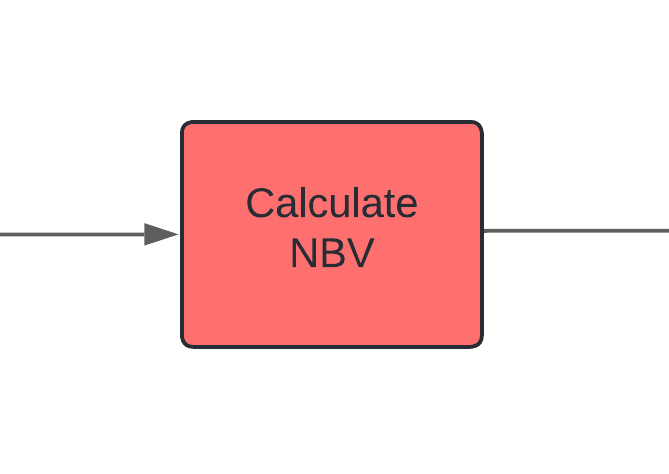
\includegraphics[width=\textwidth]{Graphics/nbv_flow.png}
	\end{textblock*}

\end{frame}


\begin{frame}{Schritt 1 \& 2}

	\begin{block}{1. Breitensuche: Frontier-Voxel und Oberflächen-Voxel}
		\begin{itemize}
			\item Finde alle besetzen Voxel, die über besetze Voxel mit Origin verbunden sind
			\item Findet die bisher bekannte Oberfläche
			\item Filtert den Boden heraus
			\item Markiert alle gefundenen unbekannte Voxel die freien Nachbarn haben
		\end{itemize}
	\end{block}
	\begin{exampleblock}{2. Breitensuche: Frontier Voxel gruppieren}
		\begin{itemize}
			\item 2 verschachtelte Breitensuchen
			\item gruppiert alle benachbarten Frontier Voxel zu einer Frontier
			\item Berechnet Zentrum der Frontier
		\end{itemize}
	\end{exampleblock}
\end{frame}

\begin{frame}
	\vspace{-0.4cm}
	\begin{figure}
		\centering
		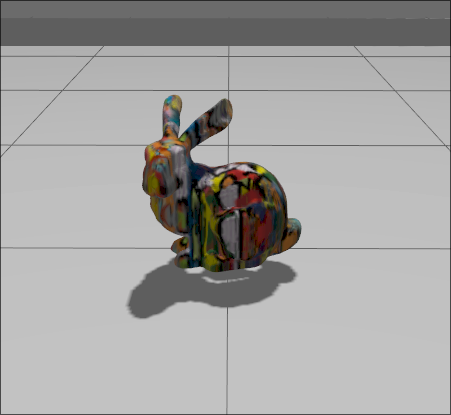
\includegraphics[width=0.4\textwidth]{Graphics/bunny.png}
		\caption{Bunny collada file provided by \cite{delmerico_comparison_2018}}
	\end{figure}
	\vspace{-0.2cm}
	\begin{minipage}{0.49\textwidth}
		\centering
		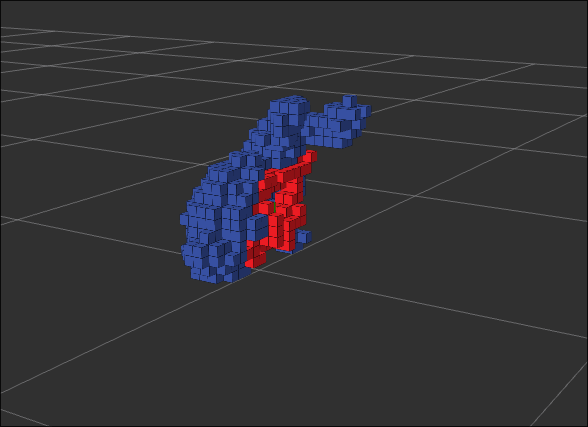
\includegraphics[width=\textwidth]{Graphics/voxel_side.png}
	\end{minipage}
	%\end{center}
	\hfill
	\begin{minipage}{0.49\textwidth}
		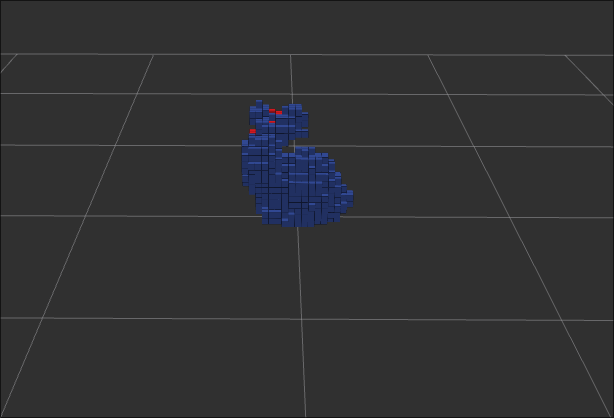
\includegraphics[width=\textwidth]{Graphics/voxel_front.png}
	\end{minipage}

\end{frame}
\begin{frame}{Schritt 3: Kandidaten Positionen generieren}
	\begin{block}{}

		\begin{center}
			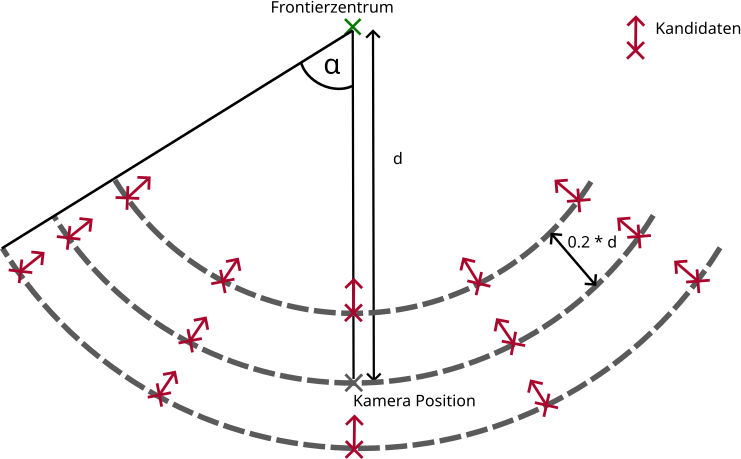
\includegraphics[width=0.7\textwidth]{Graphics/view_point_gen_v2.png}
		\end{center}
		\begin{itemize}
			\item Sampling zwischen fixen Distanzen, abhängig von aktueller Distanz $d$
			\item Sampling zwischen maximalem Ausschlagswinkel $\alpha$
			\item Alle Kandidaten werden evaluiert
		\end{itemize}
	\end{block}

\end{frame}

\begin{frame}{Schritt 4: Evaluation}
	\begin{block}{}
		Folgende Faktoren werden für die Utility Function gewertet:
		\begin{itemize}
			\item $n_{u}$ Anzahl getroffener visible unknown Voxel, (Raytracing)
			\item $n_s$ Anzahl Oberflächen-Voxel im Sichtkörper,
			\item $d(v)$ Distanz zur Kandidatenpose
			\item $p(v) \in \{0,1\}$ Erreichbarkeit der Kandidatenpose
		\end{itemize}
	\end{block}
\end{frame}
\section{Herausforderungen}
\begin{frame}{Herausforderung: Unknown Barrier}
	\begin{block}{}
		\begin{center}
			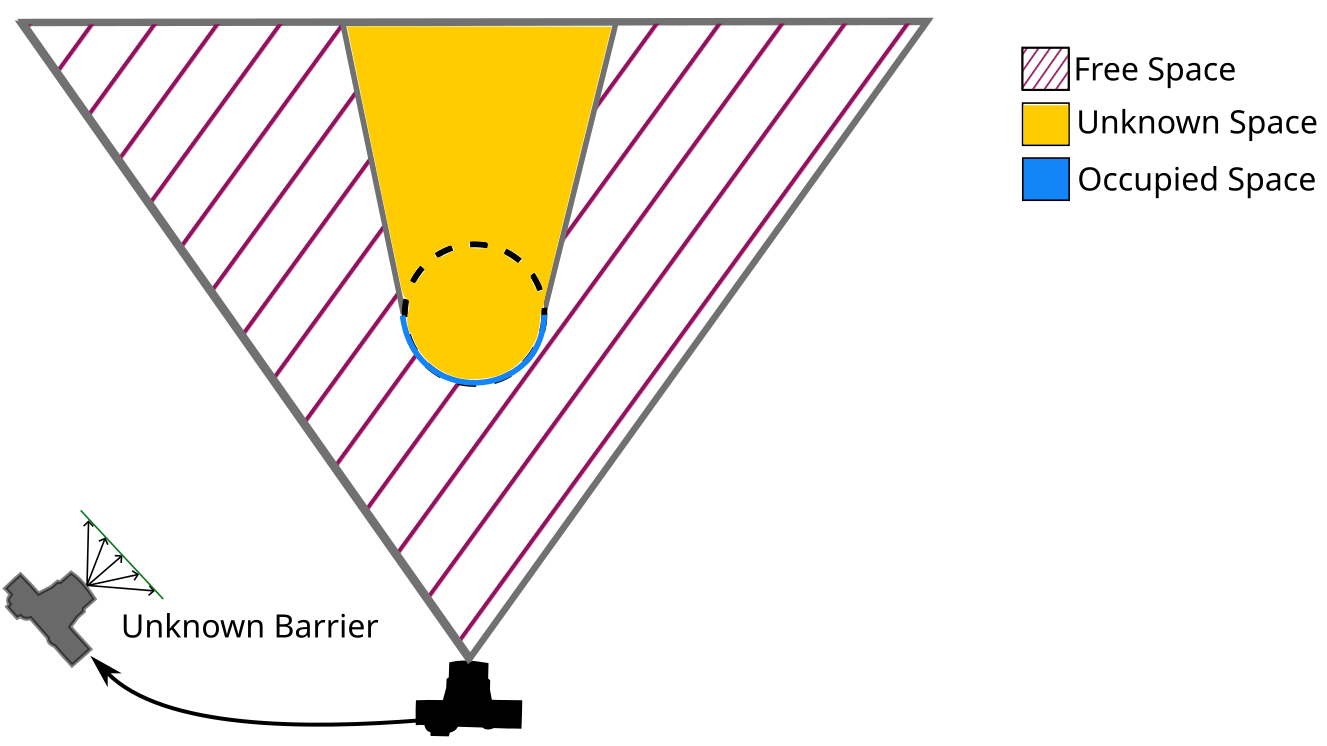
\includegraphics[width=0.7\textwidth]{Graphics/unknown_barrier_vscott_1.png}
		\end{center}
		\begin{itemize}
			\item Alle Strahlen von neuer Kamera Position treffen auf unbekannte Voxel
			\item Interessanter Bereich hinter Object minimieren
		\end{itemize}
	\end{block}
\end{frame}

\begin{frame}{Herausforderung: Unknown Barrier}
	\begin{block}{}
		\begin{center}
			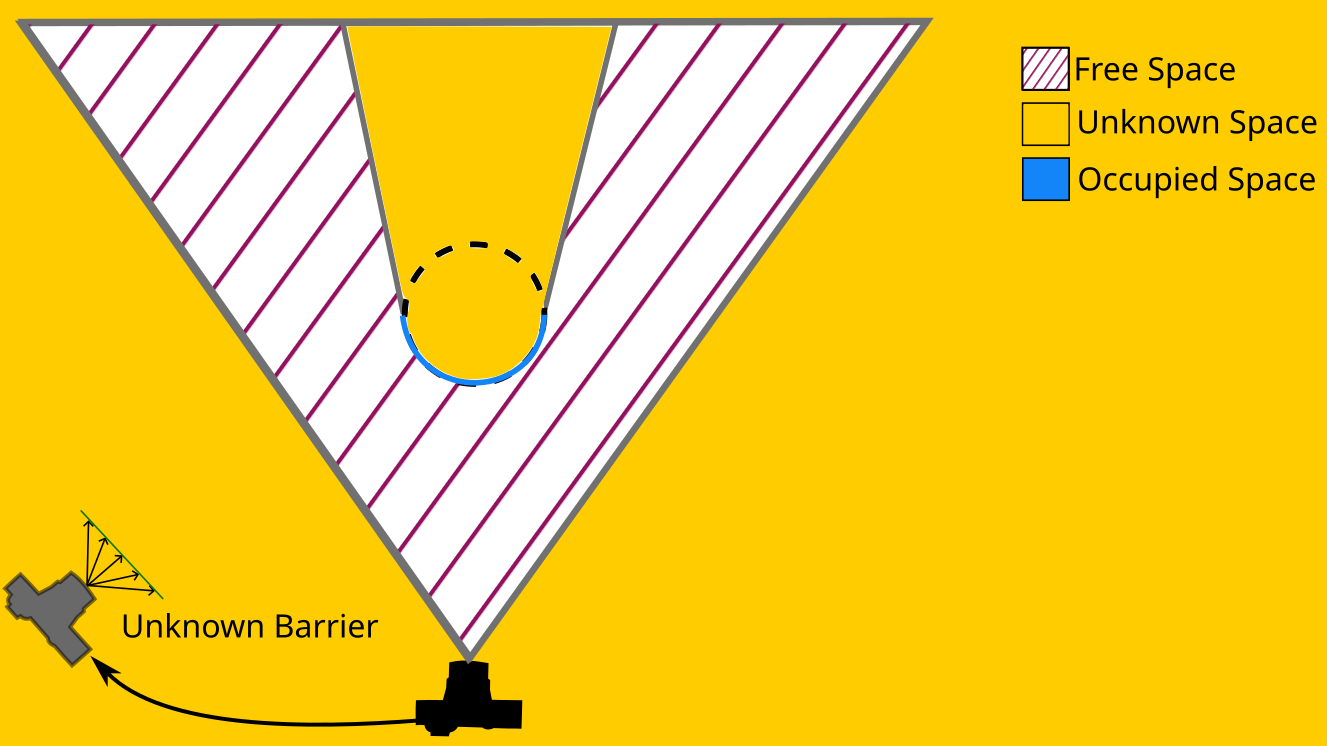
\includegraphics[width=0.7\textwidth]{Graphics/unknown_barrier_vscott_2.png}
		\end{center}
		\begin{itemize}
			\item Alle Strahlen von neuer Kamera Position treffen auf unbekannte Voxel
			\item Interessanter Bereich hinter Object minimieren
		\end{itemize}
	\end{block}
\end{frame}
\begin{frame}{Herausforderung: Unknown Barrier}
	\begin{block}{}
		\begin{center}
			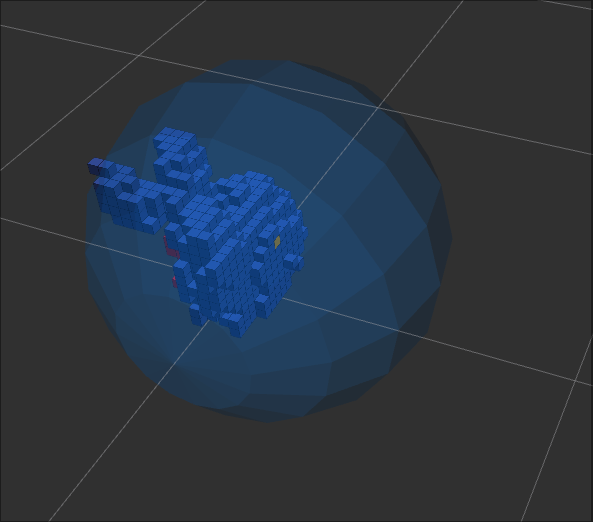
\includegraphics[width=0.4\textwidth]{Graphics/sphere.png}
		\end{center}
		\begin{itemize}
			\item \textbf{Vorübergehende Lösung:} Kugel um Origin mit Radius maximal Abstand zu einem Oberflächenvoxel
			\item \textbf{Vorteil:} Einfaches Raytracing, einfach zu berechnende Heuristik
			\item \textbf{Nachteil:} Vermutlich zu starke Heuristik, vor allem für unsymmetrische Objekte
		\end{itemize}
	\end{block}
\end{frame}
\begin{frame}{}
	\centering
	\Large{Danke für die Aufmerksamkeit!}
	\vfill
	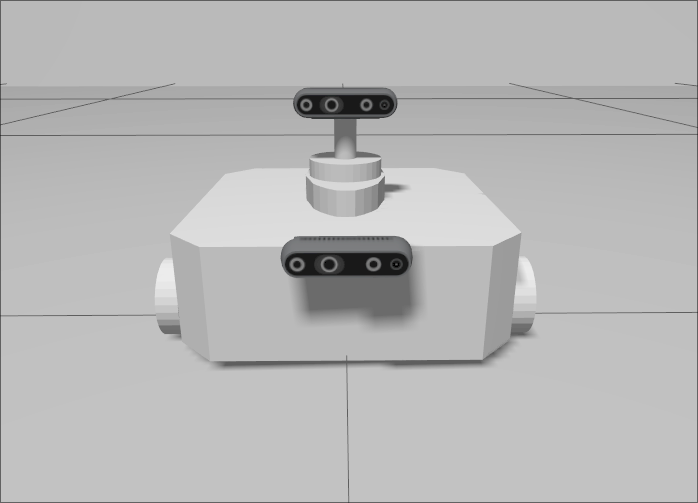
\includegraphics[width=0.5\textwidth]{Graphics/tb.png}
\end{frame}

\printbibliography
\end{document}
